\documentclass[12pt, openany]{report}
\usepackage[utf8]{inputenc}
\usepackage[T1]{fontenc}
\usepackage{amsmath,amsfonts,amssymb}
\usepackage{amssymb}
\usepackage{multicol}
\usepackage[a4paper,left=2.5cm,right=2.5cm,top=2.5cm,bottom=2.5cm]{geometry}
\usepackage[english]{babel}
\usepackage{libertine}
\usepackage{graphicx}
\usepackage{wrapfig}
\usepackage{algorithm}
\usepackage{algpseudocode}
\usepackage{float}
\usepackage{enumitem}
\usepackage{pythonhighlight}
\usepackage[]{titletoc}
\usepackage{empheq}
\usepackage{titlesec}
\usepackage{mathpazo}
\usepackage{xfrac}
\usepackage{textcomp}
\usepackage{mathtools}
\usepackage{caption}
\usepackage{tabularray}
\usepackage{subcaption}
\usepackage[bottom]{footmisc}
\usepackage{pdfpages}
\usepackage{tabularx}
\usepackage{amsthm}
\usepackage[skins]{tcolorbox}
\titleformat{\chapter}[display]
  {\normalfont\bfseries}{}{0pt}{\Huge}
\usepackage{hyperref}
\newcommand{\hsp}{\hspace{20pt}}
\newcommand{\HRule}{\rule{\linewidth}{0.5mm}}
\newcommand{\R}{\mathbb{R}}
\newcommand{\C}{\mathbb{C}}
\newcommand{\A}{\mathcal{A}}
\theoremstyle{definition}
\newtheorem{thm}{Theorem}[chapter]
\newtheorem{definition}[thm]{Definition}
\newtheorem{lem}[thm]{Lemma}

\hbadness=100000
\begin{document}
\begin{titlepage}
    \begin{sffamily}
    \begin{center}
        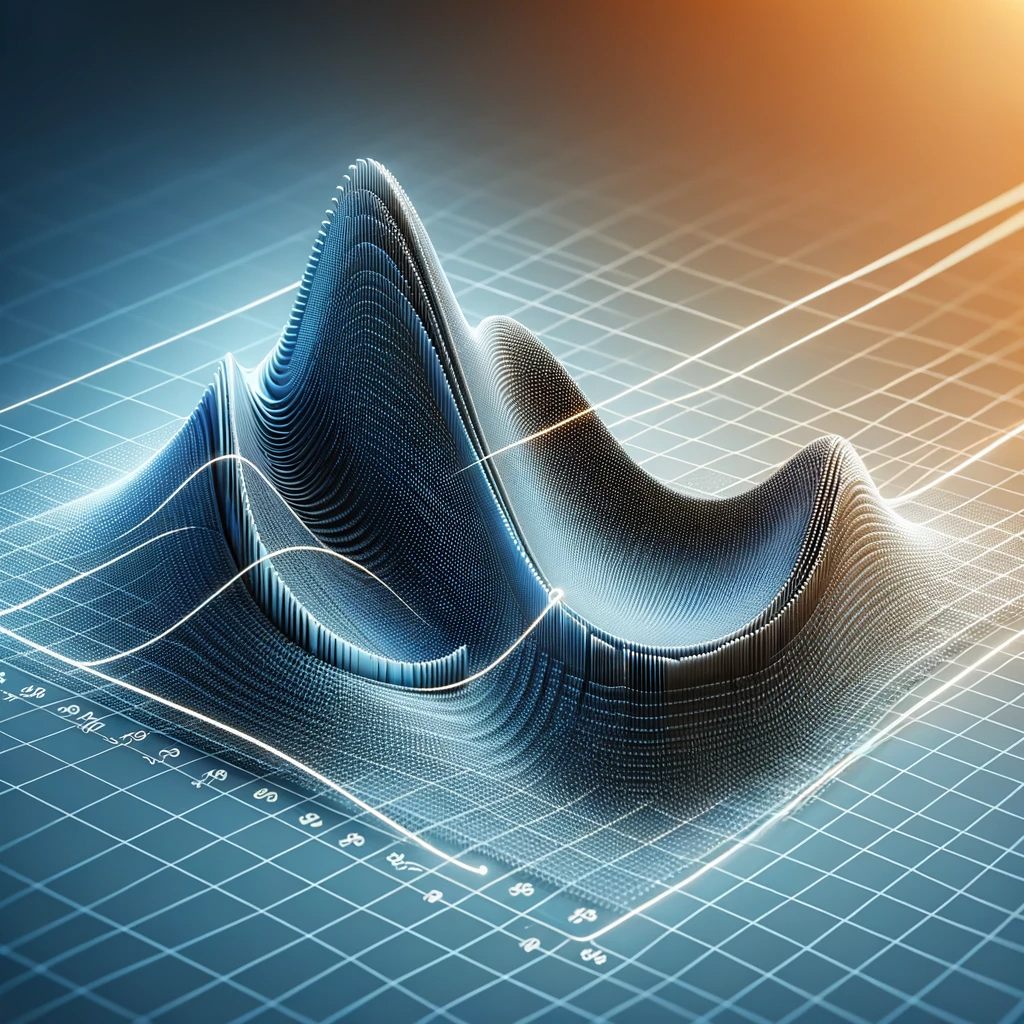
\includegraphics[scale=0.25]{img/page_de_garde.png} \\[1cm]
        \HRule \\[0.4cm]
        { \huge \bfseries LINMA2491 Operational Research \\[0.4cm] }
    
        \HRule \\[1.5cm]
        \textsc{\LARGE Simon Desmidt\\ Issambre L'Hermite Dumont}\\[1cm]
        \vfill
        \vspace{2cm}
        {\large Academic year 2024-2025 - Q2}
        \vspace{0.4cm}
         
        
\includegraphics[width=0.15\textwidth]{img/epl.png}
        
        UCLouvain\\
    
    \end{center}
    \end{sffamily}
\end{titlepage}

\setcounter{tocdepth}{1}
\tableofcontents
\chapter{Definition and notation}
\begin{itemize}
	\item Given $\Omega$, a sigma-algebra $\A$ is a set of subsets of $\Omega$, with the elements called events, such that:
	\begin{itemize}
		\item $\Omega \in \A$
		\item if $A \in \A$ then also $\Omega - A \in \A$
		\item if $A_i \in \A$ for $i = 1,2, \dots$ then also $\cup_{i=1}^\infty A_i \in \A$
		\item if $A_i \in \A$ for $i = 1,2, \dots$ then also $\cap_{i=1}^\infty A_i \in \A$
	\end{itemize}
	\item Consider: 
	\begin{figure}[H]
		\centering
		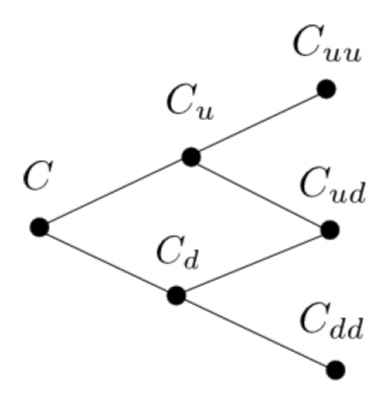
\includegraphics[scale=0.25]{img/space.jpg} 
	\end{figure}
	\begin{itemize}
		\item The state space is the set of all values of the system at each stage. 
		\begin{equation}
			S_0 = \{C\},\quad S_1 = \{C_u, C_d\},\quad S_2 = \{C_{uu}, C_{ud}, C_{dd}\}
		\end{equation}
		\item  The sample space is the set of all possible combination of the system.
		\begin{equation}
			\Omega = S_0 \times S_1 \times S_2 = \{(C, C_u, C_{uu}), (C, C_u, C_{ud}), (C, C_u, C_{dd}), \dots\}
		\end{equation}
	\end{itemize}
	\item The power set of $\Omega$ is the set of all of the subsets, denoted $\mathcal{B}(\Omega)$.
	\item The probability space is the triplet $(\Omega, \A, P)$ where $P$ is a probability measure.
	\begin{itemize}
		\item $P(\emptyset) = 0$
		\item $P(\Omega) = 1$
		\item $P(\cup_{i=1}^\infty A_i) = \sum_i P(A_i)$ if $A_i$ are disjoint
	\end{itemize} 
	\item $\forall t, A_t$ is the set of events on which we have information at stage $t$. For example, $A_0 = \{C\}$, $A_1 = \{C, C_u, C_d\}$. Thus is it evident that $ t_1 \leq t_2 \Rightarrow \A_{t_1} \subseteq \A_{t_2}$
	\item Consider the following problem with $x \in \R^n$ and domain $\mathcal{D}$:
	\begin{equation}
		\begin{aligned}
			&min f_0(x), \quad s.t.\\
			&f_i(x) \leq 0, i = 1, \dots, m\\
			&h_j(x) = 0, j = 1, \dots, p
		\end{aligned}
	\end{equation}
	Then the Lagrangian function is defined as $L: \R^n \times \R^m \times \R^p \to \R$:
	\begin{equation}
		L(x, \lambda, \nu) = f_0(x) + \sum_{i=1}^m \lambda_i f_i(x) + \sum_{j=1}^p \nu_j h_j(x)
	\end{equation}
	\item  The Lagrange dual function is defined as $g: \R^m \times \R^p \to \R$:
	\begin{equation}
		g(\lambda, \nu) = \inf_{x \in \mathcal{D}} L(x, \lambda, \nu)
	\end{equation}
	\item \textcolor{red}{TODO: suite, stopped at CM1 (background), slide 35}
\end{itemize}
\chapter{TO DO}
\end{document}